%% LyX 2.3.7 created this file.  For more info, see http://www.lyx.org/.
%% Do not edit unless you really know what you are doing.
\documentclass[english,journal,article,submit,pdftex,moreauthors]{mdpi}
\usepackage{array}
\usepackage{float}
\usepackage{url}
\usepackage{graphicx}

\makeatletter

%%%%%%%%%%%%%%%%%%%%%%%%%%%%%% LyX specific LaTeX commands.

\Title{An intelligent technique for initial distribution of genetic algorithms}

\TitleCitation{An intelligent technique for initial distribution of genetic algorithms}

\newcommand{\orcidauthorA}{0000-0000-0000-000X}


\newcommand{\orcidauthorB}{0000-0000-0000-000X}


\Author{Vasileios Charilogis$^{2}$, Ioannis G. Tsoulos$^{1,*}$, Vasileios
Stavrou$^{3}$}

\AuthorNames{Vasileios Tsoulos, Ioannis G. Tsoulos, Vasileios Stavrou }

\AuthorCitation{Charilogis, V; Tsoulos I.G.; Stavrou V.N.}


\address{$^{1}$\quad{}Department of Informatics and Telecommunications,
University of Ioannina, Greece; itsoulos@uoi.gr\\
$^{2}$\quad{}Department of Informatics and Telecommunications, University
of Ioannina, Greece; v.charilog@uoi.gr\\
$^{3}\quad$Hellenic Naval Academy, Department of Computer Science,
Military Institutions of University Education, 18539 Piraeus, Greece}


\corres{Correspondence: itsoulos@uoi.gr;}


\firstnote{Current address: Department of Informatics and Telecommunications,
University of Ioannina, Greece.}


\secondnote{These authors contributed equally to this work.}


\abstract{The need to find the global minimum in multivariable functions is
a critical problem in many fields of science and technology. Effectively
solving this problem requires the creation of initial solution estimates,
which are subsequently used by the optimization algorithm to search
for the best solution in the solution space. In the context of this
article, a novel approach to generating the initial solution distribution
is presented which is applied to a genetic optimization algorithm.
Using the k-means clustering algorithm, a distribution based on data
similarity is created. This helps in generating initial estimates
that may be more tailored to the problem. Additionally, the proposed
method employs a rejection sampling algorithm to discard samples that
do not yield better solution estimates in the optimization process.
This allows the algorithm to focus on potentially optimal solutions,
thus improving its performance. Finally, the article presents experimental
results from the application of this approach to various optimization
problems, providing the scientific community with a new method for
addressing this significant problem.}


\keyword{Optimization, Genetic algorithm methods, \textgreek{I}nitialization
distribution,Evolutionary techniques, Stochastic methods, Termination
rules.}

\DeclareFontEncoding{LGR}{}{}
\DeclareRobustCommand{\greektext}{%
  \fontencoding{LGR}\selectfont\def\encodingdefault{LGR}}
\DeclareRobustCommand{\textgreek}[1]{\leavevmode{\greektext #1}}
\ProvideTextCommand{\~}{LGR}[1]{\char126#1}

\DeclareTextSymbolDefault{\textquotedbl}{T1}
%% Because html converters don't know tabularnewline
\providecommand{\tabularnewline}{\\}
\floatstyle{ruled}
\newfloat{algorithm}{tbp}{loa}
\providecommand{\algorithmname}{Algorithm}
\floatname{algorithm}{\protect\algorithmname}

%%%%%%%%%%%%%%%%%%%%%%%%%%%%%% User specified LaTeX commands.
%  LaTeX support: latex@mdpi.com 
%  For support, please attach all files needed for compiling as well as the log file, and specify your operating system, LaTeX version, and LaTeX editor.

%=================================================================


% For posting an early version of this manuscript as a preprint, you may use "preprints" as the journal and change "submit" to "accept". The document class line would be, e.g., \documentclass[preprints,article,accept,moreauthors,pdftex]{mdpi}. This is especially recommended for submission to arXiv, where line numbers should be removed before posting. For preprints.org, the editorial staff will make this change immediately prior to posting.

%--------------------
% Class Options:
%--------------------
%----------
% journal
%----------
% Choose between the following MDPI journals:
% acoustics, actuators, addictions, admsci, adolescents, aerospace, agriculture, agriengineering, agronomy, ai, algorithms, allergies, alloys, analytica, animals, antibiotics, antibodies, antioxidants, applbiosci, appliedchem, appliedmath, applmech, applmicrobiol, applnano, applsci, aquacj, architecture, arts, asc, asi, astronomy, atmosphere, atoms, audiolres, automation, axioms, bacteria, batteries, bdcc, behavsci, beverages, biochem, bioengineering, biologics, biology, biomass, biomechanics, biomed, biomedicines, biomedinformatics, biomimetics, biomolecules, biophysica, biosensors, biotech, birds, bloods, blsf, brainsci, breath, buildings, businesses, cancers, carbon, cardiogenetics, catalysts, cells, ceramics, challenges, chemengineering, chemistry, chemosensors, chemproc, children, chips, cimb, civileng, cleantechnol, climate, clinpract, clockssleep, cmd, coasts, coatings, colloids, colorants, commodities, compounds, computation, computers, condensedmatter, conservation, constrmater, cosmetics, covid, crops, cryptography, crystals, csmf, ctn, curroncol, currophthalmol, cyber, dairy, data, dentistry, dermato, dermatopathology, designs, diabetology, diagnostics, dietetics, digital, disabilities, diseases, diversity, dna, drones, dynamics, earth, ebj, ecologies, econometrics, economies, education, ejihpe, electricity, electrochem, electronicmat, electronics, encyclopedia, endocrines, energies, eng, engproc, ent, entomology, entropy, environments, environsciproc, epidemiologia, epigenomes, est, fermentation, fibers, fintech, fire, fishes, fluids, foods, forecasting, forensicsci, forests, foundations, fractalfract, fuels, futureinternet, futureparasites, futurepharmacol, futurephys, futuretransp, galaxies, games, gases, gastroent, gastrointestdisord, gels, genealogy, genes, geographies, geohazards, geomatics, geosciences, geotechnics, geriatrics, hazardousmatters, healthcare, hearts, hemato, heritage, highthroughput, histories, horticulturae, humanities, humans, hydrobiology, hydrogen, hydrology, hygiene, idr, ijerph, ijfs, ijgi, ijms, ijns, ijtm, ijtpp, immuno, informatics, information, infrastructures, inorganics, insects, instruments, inventions, iot, j, jal, jcdd, jcm, jcp, jcs, jdb, jeta, jfb, jfmk, jimaging, jintelligence, jlpea, jmmp, jmp, jmse, jne, jnt, jof, joitmc, jor, journalmedia, jox, jpm, jrfm, jsan, jtaer, jzbg, kidney, kidneydial, knowledge, land, languages, laws, life, liquids, literature, livers, logics, logistics, lubricants, lymphatics, machines, macromol, magnetism, magnetochemistry, make, marinedrugs, materials, materproc, mathematics, mca, measurements, medicina, medicines, medsci, membranes, merits, metabolites, metals, meteorology, methane, metrology, micro, microarrays, microbiolres, micromachines, microorganisms, microplastics, minerals, mining, modelling, molbank, molecules, mps, msf, mti, muscles, nanoenergyadv, nanomanufacturing, nanomaterials, ncrna, network, neuroglia, neurolint, neurosci, nitrogen, notspecified, nri, nursrep, nutraceuticals, nutrients, obesities, oceans, ohbm, onco, oncopathology, optics, oral, organics, organoids, osteology, oxygen, parasites, parasitologia, particles, pathogens, pathophysiology, pediatrrep, pharmaceuticals, pharmaceutics, pharmacoepidemiology, pharmacy, philosophies, photochem, photonics, phycology, physchem, physics, physiologia, plants, plasma, pollutants, polymers, polysaccharides, poultry, powders, preprints, proceedings, processes, prosthesis, proteomes, psf, psych, psychiatryint, psychoactives, publications, quantumrep, quaternary, qubs, radiation, reactions, recycling, regeneration, religions, remotesensing, reports, reprodmed, resources, rheumato, risks, robotics, ruminants, safety, sci, scipharm, seeds, sensors, separations, sexes, signals, sinusitis, skins, smartcities, sna, societies, socsci, software, soilsystems, solar, solids, sports, standards, stats, stresses, surfaces, surgeries, suschem, sustainability, symmetry, synbio, systems, taxonomy, technologies, telecom, test, textiles, thalassrep, thermo, tomography, tourismhosp, toxics, toxins, transplantology, transportation, traumacare, traumas, tropicalmed, universe, urbansci, uro, vaccines, vehicles, venereology, vetsci, vibration, viruses, vision, waste, water, wem, wevj, wind, women, world, youth, zoonoticdis 

%---------
% article
%---------
% The default type of manuscript is "article", but can be replaced by: 
% abstract, addendum, article, book, bookreview, briefreport, casereport, comment, commentary, communication, conferenceproceedings, correction, conferencereport, entry, expressionofconcern, extendedabstract, datadescriptor, editorial, essay, erratum, hypothesis, interestingimage, obituary, opinion, projectreport, reply, retraction, review, perspective, protocol, shortnote, studyprotocol, systematicreview, supfile, technicalnote, viewpoint, guidelines, registeredreport, tutorial
% supfile = supplementary materials

%----------
% submit
%----------
% The class option "submit" will be changed to "accept" by the Editorial Office when the paper is accepted. This will only make changes to the frontpage (e.g., the logo of the journal will get visible), the headings, and the copyright information. Also, line numbering will be removed. Journal info and pagination for accepted papers will also be assigned by the Editorial Office.

%------------------
% moreauthors
%------------------
% If there is only one author the class option oneauthor should be used. Otherwise use the class option moreauthors.

%---------
% pdftex
%---------
% The option pdftex is for use with pdfLaTeX. If eps figures are used, remove the option pdftex and use LaTeX and dvi2pdf.

%=================================================================
% MDPI internal commands
\firstpage{1} 
 
\setcounter{page}{\@firstpage} 

\pubvolume{1}
\issuenum{1}
\articlenumber{0}
\pubyear{2022}
\copyrightyear{2022}
%\externaleditor{Academic Editor: Firstname Lastname} % For journal Automation, please change Academic Editor to "Communicated by"
\datereceived{} 
\dateaccepted{} 
\datepublished{} 
%\datecorrected{} % Corrected papers include a "Corrected: XXX" date in the original paper.
%\dateretracted{} % Corrected papers include a "Retracted: XXX" date in the original paper.
\hreflink{https://doi.org/} % If needed use \linebreak
%\doinum{}
%------------------------------------------------------------------
% The following line should be uncommented if the LaTeX file is uploaded to arXiv.org
%\pdfoutput=1

%=================================================================
% Add packages and commands here. The following packages are loaded in our class file: fontenc, inputenc, calc, indentfirst, fancyhdr, graphicx, epstopdf, lastpage, ifthen, lineno, float, amsmath, setspace, enumitem, mathpazo, booktabs, titlesec, etoolbox, tabto, xcolor, soul, multirow, microtype, tikz, totcount, changepage, attrib, upgreek, cleveref, amsthm, hyphenat, natbib, hyperref, footmisc, url, geometry, newfloat, caption

%=================================================================
%% Please use the following mathematics environments: Theorem, Lemma, Corollary, Proposition, Characterization, Property, Problem, Example, ExamplesandDefinitions, Hypothesis, Remark, Definition, Notation, Assumption
%% For proofs, please use the proof environment (the amsthm package is loaded by the MDPI class).

%=================================================================
% The fields PACS, MSC, and JEL may be left empty or commented out if not applicable
%\PACS{J0101}
%\MSC{}
%\JEL{}

%%%%%%%%%%%%%%%%%%%%%%%%%%%%%%%%%%%%%%%%%%
% Only for the journal Diversity
%\LSID{\url{http://}}

%%%%%%%%%%%%%%%%%%%%%%%%%%%%%%%%%%%%%%%%%%
% Only for the journal Applied Sciences:
%\featuredapplication{Authors are encouraged to provide a concise description of the specific application or a potential application of the work. This section is not mandatory.}
%%%%%%%%%%%%%%%%%%%%%%%%%%%%%%%%%%%%%%%%%%

%%%%%%%%%%%%%%%%%%%%%%%%%%%%%%%%%%%%%%%%%%
% Only for the journal Data:
%\dataset{DOI number or link to the deposited data set in cases where the data set is published or set to be published separately. If the data set is submitted and will be published as a supplement to this paper in the journal Data, this field will be filled by the editors of the journal. In this case, please make sure to submit the data set as a supplement when entering your manuscript into our manuscript editorial system.}

%\datasetlicense{license under which the data set is made available (CC0, CC-BY, CC-BY-SA, CC-BY-NC, etc.)}

%%%%%%%%%%%%%%%%%%%%%%%%%%%%%%%%%%%%%%%%%%
% Only for the journal Toxins
%\keycontribution{The breakthroughs or highlights of the manuscript. Authors can write one or two sentences to describe the most important part of the paper.}

%%%%%%%%%%%%%%%%%%%%%%%%%%%%%%%%%%%%%%%%%%
% Only for the journal Encyclopedia
%\encyclopediadef{Instead of the abstract}
%\entrylink{The Link to this entry published on the encyclopedia platform.}
%%%%%%%%%%%%%%%%%%%%%%%%%%%%%%%%%%%%%%%%%%

\makeatother

\usepackage{babel}
\begin{document}
\maketitle

\section{Introduction}

The task of locating the global minimum of a function $f$ can be
defined as:
\begin{equation}
x^{*}=\mbox{arg}\min_{x\in S}f(x)\label{eq:eq1}
\end{equation}
with $S$: 
\[
S=\left[a_{1},b_{1}\right]\times\left[a_{2},b_{2}\right]\times\ldots\left[a_{n},b_{n}\right]
\]
This task finds application in a variety of real world problems, such
as problems from physics \citep{go_physics1,go_physics2,go_physics3},
chemistry \citep{go_chem1,go_chem2,go_chem3}, economics \citep{go_econ1,go_econ2},
medicine \citep{go_med1,go_med2} etc. The methods aimed at finding
the global minimum are divided into two major categories: deterministic
methods and stochastic methods. The most frequently encountered techniques
of the first category are interval techniques \citep{interval1,interval2},
which partition the initial domain of the objective function until
a promising subset is found to find the global minimum. The second
category includes the vast majority of methods and in its ranks one
can find methods such as Controlled Random Search methods \citep{crs1,crs2,crs3},
Simulated Annealing methods \citep{simann_major,simann1,simann2},
Differential Evolution methods \citep{diffe1,diffe2}, Particle Swarm
Optimization (PSO) methods \citep{pso_major,pso1,pso2}, Ant Colony
optimization methods \citep{aco1,aco2}, etc. Furthermore, a variety
of hybrid techniques have been proposed, such as hybrid Multistart
methods \citep{mshybrid1,mshybrid2}, hybrid PSO techniques \citep{psohybrid1,psohybrid2,psohybrid3}
etc. Also, many parallel optimization methods \citep{parallel-multistart,parallel-multistart2}
have appeared during the past years or methods that take advantage
of the modern graphics processing units (GPU) \citep{msgpu1,msgpu2}.

One of the basic techniques included in the area of stochastic techniques
is Genetic Algorithms, initially proposed by John Holland \citep{Holland1}.
The operation of genetic algorithms is inspired by biology, and for
this reason, it utilizes the idea of evolution through genetic mutation,
natural selection, and crossover \citep{Stender,genetic1,genetic2}. 

Genetic algorithms can be combined with machine learning to solve
complex problems and optimize models. More specifically, the genetic
algorithm has been applied in many machine learning applications,
such as in the article by Ansari et al, which deals with the recognition
of digital modulation signals. In this article, the genetic algorithm
is used to optimize machine learning models by adjusting their features
and parameters to achieve better signal recognition accuracy \citep{Ansari}.
Additionally, in the study by Ji et al, a methodology is proposed
that uses machine learning models to predict amplitude deviation in
hot rolling, while genetic algorithms are employed to optimize the
machine learning models and select features to improve prediction
accuracy \citep{Ji}. Furthermore, in the article by Santana, Alonso,
and Nieto, which focuses on the design and optimization of 5G networks
in indoor environments, the use of genetic algorithms and machine
learning models is identified for estimating path loss, which is critical
for determining signal strength and coverage indoors \citep{Santana}.

Another interesting article is by Liu et al, which discusses the use
of genetic algorithms in robotics \citep{Liu}. The authors propose
a methodology that utilizes genetic algorithms to optimize the trajectory
and motion of digital twin robots. A similar study was presented by
Nonoyama et al \citep{Nonoyama}, where the research focused on optimizing
energy consumption during the motion planning of a dual-arm industrial
robot. The goal of the research is to minimize energy consumption
during the process of object retrieval and placement. To achieve this,
both genetic algorithms and particle swarm optimization algorithms
are used to adjust the robot's motion trajectory, thereby increasing
its energy efficiency.

The use of genetic algorithms is still prevalent even in the business
world. In the article by Liu et al \citep{LiuK}, the application
of genetic algorithms in an effort to optimize energy conservation
in a high-speed Methanol Spark Ignition engine fueled with Methanol
and gasoline blends is discussed. In this study, genetic algorithms
were used as an optimization technique to find the best operating
conditions for the engine, such as the air-fuel ratio, ignition timing,
and other engine control variables, aiming to save energy and reduce
energy consumption and emissions. In another research, the optimization
of the placement of electric vehicle charging stations is carried
out \citep{Zhou}. Furthermore, in the study by Chen and Hu \citep{Chen},
the design of an intelligent system for agricultural greenhouses using
genetic algorithms is presented to provide multiple energy sources.
Similarly, in the research by Min, Song, Chen, Wang, and Zhang \citep{Min},
an optimized energy management strategy for hybrid electric vehicles
is introduced using a genetic algorithm based on fuel cells in a neural
network under startup conditions.

Moreover, genetic algorithms are extremely useful in the field of
medicine, as they are employed in therapy optimization, medical personnel
training, genetic diagnosis, and genomic research. More specifically,
in the study by Doewes, Nair \& Sharma \citep{Doewes}, data from
blood analyses and other biological samples were used to extract characteristics
related to the presence of the SARS-CoV-2 virus that causes COVID-19.
In this article, genetic algorithms are used for data analysis and
processing to extract significant characteristics that can aid in
the effective diagnosis of COVID-19. Additionally, there are studies
that present the design of dental implants for patients using artificial
neural networks and genetic algorithms \citep{Choudhury}, \citep{ElAnwar}.
Lastly, the contribution of genetic algorithms is significant in both
implant techniques \citep{Zheng}, \citep{Brahim} and surgeries \citep{Tokgoz},
\citep{Wang}.

The current work aims to improve the efficiency of the genetic algorithm
in global optimization problems, by introducing a new way of initializing
the population's chromosomes. In the new initialization technique,
the k-means \citep{kmeansNew} method is used to find initial values
of the chromosomes that will lead to finding the global minimum faster
and more efficient than chromosomes generated by some random distribution.
Also, the proposed technique discards chromosomes which, after applying
the k-means technique, are close to each other.

During the past years, many researchers have proposed variations for
the initialization of genetic algorithms, such as the work of Maaranen
et al \citep{gainit1}, where they discuss the usage of quasi-random
sequences in the initial population of a genetic algorithm. Similarly,
Paul et al \citep{gainit2} proposed initializing the population of
genetic algorithm using a Vari-begin and Vari-diversity (VV) population
seeding technique. Also, in the same direction of research, Li et
al proposed \citep{gainit3} a knowledge-based technique to initialize
genetic algorithms used mainly in discrete problems. Recently, Hassanat
et al suggested the incorporation of regression techniques for the
initialization of genetic algorithms. 

The rest of this article is organized as follows: in section \ref{sec:The-proposed-method}
the proposed method is discussed in detail, in section \ref{sec:Experiments}
the used test functions as well the experimental results are fully
outlined and finally in section \ref{sec:Conclusions} some conclusions
and future guidelines are listed.

\section{The proposed method\label{sec:The-proposed-method}}

The fundamental operation of a genetic algorithm mimics the process
of natural evolution. The algorithm begins by creating an initial
population of solutions, called chromosomes that represents a potential
solution to the objective problem. The genetic algorithm operates
by reproducing and evolving populations of solutions through iterative
steps. Following the analogy to natural evolution, the genetic algorithm
allows optimal solutions to \textquotedbl evolve\textquotedbl{} through
successive generations. The main steps of the used genetic algorithm
are described below:
\begin{enumerate}
\item \textbf{Initialization Step}
\begin{enumerate}
\item \textbf{Set} $N_{c}$ as the number of chromosomes.
\item \textbf{Set} $N_{g}$ the maximum number of allowed generations. 
\item \textbf{Initialize} randomly the $N_{c}$ chromosomes in $S$. In
most implementations of genetic algorithms, the chromosomes will be
selected using some random number distribution. In the present work,
the chromosomes will be selected using the sampling technique described
in subsection \ref{subsec:The-proposed-sampling}.
\item \textbf{Set} as $p_{s}$ the selection rate of the algorithm, with
$p_{s}\le1$.
\item \textbf{Set} as $p_{m}$ the mutation rate, with $p_{m}\le1$.
\item \textbf{Set} iter=0.
\end{enumerate}
\item \textbf{For} every chromosome\textbf{ }$g_{i},\ i=1,\ldots,N_{c}$
\textbf{Calculate} the fitness $f_{i}=f\left(g_{i}\right)$ of chromosome
$g_{i}$.\textbf{\label{enu:Fitness-calculation-Step}}
\item \textbf{Genetic operations step}
\begin{enumerate}
\item \textbf{Selection procedure.} The chromosomes are sorted according
to their fitness values. Denote as $N_{b}$ the integer part of $\left(1-p_{s}\right)\times N_{c}$
chromosomes with the lowest fitness values are transferred intact
to the next generation. The remain chromosomes are substituted by
offspings created in the crossover procedure. During the selection
process for each offspring two parents are selected from the population
using the tournament selection. 
\item \textbf{Crossover procedure}: For every pair $(z,w)$ of selected
parents two additional chromosomes $\tilde{z}$ and $\tilde{w}$ are
produced using the following equations
\begin{eqnarray}
\tilde{z_{i}} & = & a_{i}z_{i}+\left(1-a_{i}\right)w_{i}\nonumber \\
\tilde{w_{i}} & = & a_{i}w_{i}+\left(1-a_{i}\right)z_{i}\label{eq:crossover_ali-1}
\end{eqnarray}
where $i=1,\ldots,n$. The values $a_{i}$ are uniformly distributed
random numbers, with $a_{i}\in[-0.5,1.5]$ \citep{kaelo}. 
\item \textbf{Replacement procedure}. 
\begin{enumerate}
\item \textbf{For} $i=N_{b}+1$ to $N_{c}$ \textbf{do}
\begin{enumerate}
\item \textbf{Replace} $g_{i}$ using the next offspring created in the
crossover procedure.
\end{enumerate}
\item \textbf{EndFor}
\end{enumerate}
\item \textbf{Mutation procedure}:\textbf{ }
\begin{enumerate}
\item \textbf{For} every chromosome $g_{i},\ i=1,\ldots,N_{c}$ do
\begin{enumerate}
\item \textbf{For} each element $\ j=1,\ldots,n$ of $g_{i}$ a uniformly
distributed random number $r\in\left[0,1\right]$ is drawn. The element
is altered randomly if $r\le p_{m}$.
\end{enumerate}
\item \textbf{EndFor} 
\end{enumerate}
\end{enumerate}
\item \textbf{Termination Check Step}
\begin{enumerate}
\item \textbf{Set} $iter=iter+1$ 
\item \textbf{If} $\mbox{iter}\ge N_{g}$ or the proposed stopping rule
of Tsoulos \citep{Tsoulos1} is hold, then goto Local Search Step,
else goto \ref{enu:Fitness-calculation-Step}.
\end{enumerate}
\item \textbf{Local Search Step. }Apply a local search procedure to chromosome
of the population with the lowest fitness value and report the obtained
minimum. In the current work the BFGS variant of Powell \citep{Powell}
was used as a local search procedure.
\end{enumerate}
The current work proposes a novel method to initiate the chromosomes,
that utilizes the well - known technique of k-means. The significance
of the initial distribution in solution finding within optimization
is essential across various domains and techniques. Apart from genetic
algorithms, the initial distribution impacts other optimization methods
like Particle Swarm Optimization (PSO)\citep{Kennedy}, Evolution
Strategies\citep{Beyer}, and neural networks\citep{LeCun}. The initial
distribution defines the starting solutions that will evolve and improve
throughout the algorithm. If the initial population contains solutions
close to the optimum, it increases the likelihood of evolved solutions
being in proximity to the optimal solution. Conversely, if the initial
population is distant from the optimum, the algorithm might need more
iterations to reach the optimal solution or even get stuck in a suboptimal
solution. In conclusion, the initial distribution influences the stability,
convergence speed, and quality of optimization algorithm outcomes.
Thus, selecting a suitable initial distribution is crucial for the
algorithm's efficiency and the discovery of the optimal solution in
a reasonable time \citep{Whitley,Eiben}. 

\subsection{Proposed initialization distribution}

The present work replaces the randomness of the initialization of
the chromosomes by using the k-means technique. More specifically,
the method takes a series of samples from the objective function and
then the k-means method is used to locate the centers of these points.
These centers can then be used as chromosomes in the genetic algorithm.

The k-means algorithm emerged in 1957 by Stuart Lloyd in the form
of Lloyd's algorithm\citep{Lloyd}, although the concept of clustering
based on distance had been introduced earlier. The name 'k-means'
was introduced around 1967 by James MacQueen\citep{MacQueen}. The
k-means algorithm is a clustering algorithm widely used in data analysis
and machine learning. Its primary objective is to partition a dataset
into k clusters, where data points within the same cluster are similar
to each other and differ from data points in other clusters. Specifically,
k-means seeks cluster centers and assigns samples to each cluster,
aiming to minimize the distance within clusters and maximize the distance
between cluster centers\citep{Jain}. The algorithm steps are presented
in algorithm \ref{alg:The-K-Means-algorithm.}

\begin{algorithm}[H]
\caption{The k-Means algorithm.\label{alg:The-K-Means-algorithm.}}

\begin{enumerate}
\item \textbf{Set} the number of clusters $k$
\item The input of the algorithm is the $N_{m}$ initial points $x_{i},\ i=1,\ldots,N_{m}$.
For the current algorithm $x_{i}$ are randomly selected samples in
$S$.
\item \textbf{Repeat}
\begin{enumerate}
\item Set $S_{j}=\left\{ \right\} ,\ j=1..k$
\item \textbf{For} every point $x_{i},\ i=1,...,N_{m}$ \textbf{do}
\begin{enumerate}
\item \textbf{Set} $j^{*}=\mbox{argmin}_{m=1}^{k}\left\{ D\left(x_{i},c_{m}\right)\right\} $,
where $D(x,y)$ is the Euclidean distance of $(x,y)$.
\item \textbf{Set} $S_{j^{*}}=S_{j^{*}}\cup\left\{ x_{i}\right\} $.
\end{enumerate}
\item \textbf{EndFor}
\item \textbf{For} every center $c_{j},\ j=1..k$ \textbf{do}
\begin{enumerate}
\item \textbf{Set} as $M_{j}$ the number of points in $S_{j}$
\item \textbf{Compute }$c_{j}$ as
\[
c_{j}=\frac{1}{M_{j}}\sum_{x_{i}\in S_{j}}x_{i}
\]
\end{enumerate}
\item \textbf{EndFor}
\end{enumerate}
\item \textbf{Stop }the algorithm, if there is no change in centers $c_{j}$.
\end{enumerate}
\end{algorithm}

The algorithm terminates when there is no change in cluster centers
between consecutive iterations, implying that the clusters have stabilized
in their final form\citep{Bishop,Hastie}.

\subsection{Chromosome rejection rule}

An additional technique for discarding chromosomes where they are
similar or close to each other is listed and applied below. Specifically,
each chromosome is extensively compared to all the other chromosomes,
and those that have very small or negligible Euclidean distance between
them are sought, implying their similarity. Subsequently, the algorithm
incorporates these chromosomes into the final initial distribution
table, while chromosomes that are not similar are discarded.

\begin{algorithm}[H]
\begin{enumerate}
\item \textbf{Set} $C$ the set of centers, $C=\left\{ c_{i},\ i=1,\ldots,k\right\} $
\item \textbf{Set} $\epsilon>0$ a small positive number
\item \textbf{For} every center $c_{i}$ \textbf{Do}
\begin{enumerate}
\item \textbf{For} every center $c_{j},\ j=1,\ldots,i-1$ \textbf{Do}
\begin{enumerate}
\item \textbf{If $\left\Vert c_{i}-c_{j}\right\Vert \le\epsilon$ then }remove
$c_{i}$ from $C$.
\end{enumerate}
\item \textbf{EndFor}
\end{enumerate}
\item \textbf{EndFor}
\item \textbf{Return} the final set of centers $C$
\end{enumerate}
\caption{Chromosome rejection rule\label{alg:Chromosome-rejection-rule}}

\end{algorithm}


\subsection{The proposed sampling procedure\label{subsec:The-proposed-sampling}}

The proposed sampling procedure has the following major steps:
\begin{enumerate}
\item \textbf{Take} $N_{m}$ random samples from the objective function
using uniform distribution
\item \textbf{Calculate} the $k$ centers of the $N_{m}$ points using the
k-means algorithm provided in algorithm \ref{alg:The-K-Means-algorithm.}.
\item \textbf{Remove} from the set of centers $C$, points that are closed
to each other.
\item \textbf{Return} the set of centers $C$ as the set of chromosomes.
\end{enumerate}

\section{Experiments \label{sec:Experiments}}

In the following, the benchmark functions used in the experiments
as well as the experimental results are presented. The test functions
used here was proposed in a variety of research papers \citep{Ali1,Floudas1}.

\subsection{Test functions}

The definition of the test functions used are given below
\begin{itemize}
\item \textbf{Bf1} (Bohachevsky 1) function:
\end{itemize}
\[
f(x)=x_{1}^{2}+2x_{2}^{2}-\frac{3}{10}\cos\left(3\pi x_{1}\right)-\frac{4}{10}\cos\left(4\pi x_{2}\right)+\frac{7}{10}
\]
with $x\in[-100,100]^{2}$. 
\begin{itemize}
\item \textbf{Bf2} (Bohachevsky 2) function: 
\[
f(x)=x_{1}^{2}+2x_{2}^{2}-\frac{3}{10}\cos\left(3\pi x_{1}\right)\cos\left(4\pi x_{2}\right)+\frac{3}{10}
\]
with $x\in[-50,50]^{2}$. 
\item \textbf{Branin} function: $f(x)=\left(x_{2}-\frac{5.1}{4\pi^{2}}x_{1}^{2}+\frac{5}{\pi}x_{1}-6\right)^{2}+10\left(1-\frac{1}{8\pi}\right)\cos(x_{1})+10$
with $-5\le x_{1}\le10,\ 0\le x_{2}\le15$. 
\item \textbf{CM} function: 
\[
f(x)=\sum_{i=1}^{n}x_{i}^{2}-\frac{1}{10}\sum_{i=1}^{n}\cos\left(5\pi x_{i}\right)
\]
where $x\in[-1,1]^{n}$. In the conducted experiments the value $n=4$
was used.
\item \textbf{Camel} function:
\[
f(x)=4x_{1}^{2}-2.1x_{1}^{4}+\frac{1}{3}x_{1}^{6}+x_{1}x_{2}-4x_{2}^{2}+4x_{2}^{4},\quad x\in[-5,5]^{2}
\]
\item \textbf{Easom} function: 
\[
f(x)=-\cos\left(x_{1}\right)\cos\left(x_{2}\right)\exp\left(\left(x_{2}-\pi\right)^{2}-\left(x_{1}-\pi\right)^{2}\right)
\]
with $x\in[-100,100]^{2}.$ 
\item \textbf{Exponential} function, defined as: 
\[
f(x)=-\exp\left(-0.5\sum_{i=1}^{n}x_{i}^{2}\right),\quad-1\le x_{i}\le1
\]
 The values $n=4,8,16,32$ were used in the executed experiments.
\item \textbf{Griewank2} function:
\[
f(x)=1+\frac{1}{200}\sum_{i=1}^{2}x_{i}^{2}-\prod_{i=1}^{2}\frac{\cos(x_{i})}{\sqrt{(i)}},\quad x\in[-100,100]^{2}
\]
\item \textbf{Griewank10} function. The function is given by the equation
\[
f(x)=\sum_{i=1}^{n}\frac{x_{i}^{2}}{4000}-\prod_{i=1}^{n}\cos\left(\frac{x_{i}}{\sqrt{i}}\right)+1
\]
with $n=10$.
\item \textbf{Gkls} function. $f(x)=\mbox{Gkls}(x,n,w)$, is a function
with $w$ local minima, described in \citep{gkls} with $x\in[-1,1]^{n}$
and $n$ a positive integer between 2 and 100. The values $n=2,3$
and $w=50$ were used in the conducted experiments.
\item \textbf{Goldstein and Price function }\\
\begin{eqnarray*}
f(x) & = & \left[1+\left(x_{1}+x_{2}+1\right)^{2}\right.\\
 &  & \left(19-14x_{1}+3x_{1}^{2}-14x_{2}+6x_{1}x_{2}+3x_{2}^{2}\right)]\times\\
 &  & [30+\left(2x_{1}-3x_{2}\right)^{2}\\
 &  & \left(18-32x_{1}+12x_{1}^{2}+48x_{2}-36x_{1}x_{2}+27x_{2}^{2}\right)]
\end{eqnarray*}
With $x\in[-2,2]^{2}$. 
\item \textbf{Hansen} function: $f(x)=\sum_{i=1}^{5}i\cos\left[(i-1)x_{1}+i\right]\sum_{j=1}^{5}j\cos\left[(j+1)x_{2}+j\right]$,
$x\in[-10,10]^{2}$ .
\item \textbf{Hartman 3} function:
\[
f(x)=-\sum_{i=1}^{4}c_{i}\exp\left(-\sum_{j=1}^{3}a_{ij}\left(x_{j}-p_{ij}\right)^{2}\right)
\]
with $x\in[0,1]^{3}$ and $a=\left(\begin{array}{ccc}
3 & 10 & 30\\
0.1 & 10 & 35\\
3 & 10 & 30\\
0.1 & 10 & 35
\end{array}\right),\ c=\left(\begin{array}{c}
1\\
1.2\\
3\\
3.2
\end{array}\right)$ and
\[
p=\left(\begin{array}{ccc}
0.3689 & 0.117 & 0.2673\\
0.4699 & 0.4387 & 0.747\\
0.1091 & 0.8732 & 0.5547\\
0.03815 & 0.5743 & 0.8828
\end{array}\right)
\]
\item \textbf{Hartman 6} function:
\[
f(x)=-\sum_{i=1}^{4}c_{i}\exp\left(-\sum_{j=1}^{6}a_{ij}\left(x_{j}-p_{ij}\right)^{2}\right)
\]
with $x\in[0,1]^{6}$ and $a=\left(\begin{array}{cccccc}
10 & 3 & 17 & 3.5 & 1.7 & 8\\
0.05 & 10 & 17 & 0.1 & 8 & 14\\
3 & 3.5 & 1.7 & 10 & 17 & 8\\
17 & 8 & 0.05 & 10 & 0.1 & 14
\end{array}\right),\ c=\left(\begin{array}{c}
1\\
1.2\\
3\\
3.2
\end{array}\right)$ and
\[
p=\left(\begin{array}{cccccc}
0.1312 & 0.1696 & 0.5569 & 0.0124 & 0.8283 & 0.5886\\
0.2329 & 0.4135 & 0.8307 & 0.3736 & 0.1004 & 0.9991\\
0.2348 & 0.1451 & 0.3522 & 0.2883 & 0.3047 & 0.6650\\
0.4047 & 0.8828 & 0.8732 & 0.5743 & 0.1091 & 0.0381
\end{array}\right)
\]
\item \textbf{Potential} function. The molecular conformation corresponding
to the global minimum of the energy of N atoms interacting via the
Lennard-Jones potential\citep{Jones} is used a test function here
and it is defined by:
\[
V_{LJ}(r)=4\epsilon\left[\left(\frac{\sigma}{r}\right)^{12}-\left(\frac{\sigma}{r}\right)^{6}\right]
\]
The values $N=3,\ 5$ were used in the conducted experiments. Also,
for the conducted experiments the values $\epsilon=1,\ \sigma=$1
were used.
\item \textbf{Rastrigin} function. 
\[
f(x)=x_{1}^{2}+x_{2}^{2}-\cos(18x_{1})-\cos(18x_{2}),\quad x\in[-1,1]^{2}
\]
\item \textbf{\emph{Rosenbrock}}\emph{ function}.\\
\[
f(x)=\sum_{i=1}^{n-1}\left(100\left(x_{i+1}-x_{i}^{2}\right)^{2}+\left(x_{i}-1\right)^{2}\right),\quad-30\le x_{i}\le30.
\]
The values $n=4,\ 8,\ 16$ were used in the conducted experiments.
\item \textbf{Shekel 5 }function.
\end{itemize}
\[
f(x)=-\sum_{i=1}^{5}\frac{1}{(x-a_{i})(x-a_{i})^{T}+c_{i}}
\]
 

with $x\in[0,10]^{4}$ and $a=\left(\begin{array}{cccc}
4 & 4 & 4 & 4\\
1 & 1 & 1 & 1\\
8 & 8 & 8 & 8\\
6 & 6 & 6 & 6\\
3 & 7 & 3 & 7
\end{array}\right),\ c=\left(\begin{array}{c}
0.1\\
0.2\\
0.2\\
0.4\\
0.4
\end{array}\right)$
\begin{itemize}
\item \textbf{Shekel 7} function.
\end{itemize}
\[
f(x)=-\sum_{i=1}^{7}\frac{1}{(x-a_{i})(x-a_{i})^{T}+c_{i}}
\]

with $x\in[0,10]^{4}$ and $a=\left(\begin{array}{cccc}
4 & 4 & 4 & 4\\
1 & 1 & 1 & 1\\
8 & 8 & 8 & 8\\
6 & 6 & 6 & 6\\
3 & 7 & 3 & 7\\
2 & 9 & 2 & 9\\
5 & 3 & 5 & 3
\end{array}\right),\ c=\left(\begin{array}{c}
0.1\\
0.2\\
0.2\\
0.4\\
0.4\\
0.6\\
0.3
\end{array}\right)$.
\begin{itemize}
\item \textbf{Shekel 10} function.
\end{itemize}
\[
f(x)=-\sum_{i=1}^{10}\frac{1}{(x-a_{i})(x-a_{i})^{T}+c_{i}}
\]
 

with $x\in[0,10]^{4}$ and $a=\left(\begin{array}{cccc}
4 & 4 & 4 & 4\\
1 & 1 & 1 & 1\\
8 & 8 & 8 & 8\\
6 & 6 & 6 & 6\\
3 & 7 & 3 & 7\\
2 & 9 & 2 & 9\\
5 & 5 & 3 & 3\\
8 & 1 & 8 & 1\\
6 & 2 & 6 & 2\\
7 & 3.6 & 7 & 3.6
\end{array}\right),\ c=\left(\begin{array}{c}
0.1\\
0.2\\
0.2\\
0.4\\
0.4\\
0.6\\
0.3\\
0.7\\
0.5\\
0.6
\end{array}\right)$. 
\begin{itemize}
\item \textbf{Sinusoidal} function: 
\[
f(x)=-\left(2.5\prod_{i=1}^{n}\sin\left(x_{i}-z\right)+\prod_{i=1}^{n}\sin\left(5\left(x_{i}-z\right)\right)\right),\quad0\le x_{i}\le\pi.
\]
The values of $n=4,8,16$ and $z=\frac{\pi}{6}$ was used in the conducted
experiments.
\item \textbf{Test2N} function:
\[
f(x)=\frac{1}{2}\sum_{i=1}^{n}x_{i}^{4}-16x_{i}^{2}+5x_{i},\quad x_{i}\in[-5,5].
\]
The function has $2^{n}$ in the specified range and in our experiments
we used $n=4,5,6,7$.
\item \textbf{Test30N} function:
\[
f(x)=\frac{1}{10}\sin^{2}\left(3\pi x_{1}\right)\sum_{i=2}^{n-1}\left(\left(x_{i}-1\right)^{2}\left(1+\sin^{2}\left(3\pi x_{i+1}\right)\right)\right)+\left(x_{n}-1\right)^{2}\left(1+\sin^{2}\left(2\pi x_{n}\right)\right)
\]
with $x\in[-10,10]$, with $30^{n}$ local minima in the search space.
For our experiments we used $n=3,4$.
\end{itemize}

\subsection{Experimental results}

The freely available software OPTIMUS was utilized for the experiments,
available at the following address: \url{https://github.com/itsoulos/OPTIMUS}(accessed
on 9 September 2023). The genetic algorithm variant of OPTIMUS package
used in the conducted experiments was the pDoubleGenetic algorithm,
that can utilize different methods for the initialization of chromosomes.
The machine used in the experiments was an AMD Ryzen 5950X with 128GB
of RAM, running the Debian Linux operating system. To ensure research
reliability, the experiments were executed 30 times for each objective
function, employing different seeds for the random generator, and
reporting the mean values. The values used for the parameters in the
experiments are listed in Table \ref{tab:expValues}. The values in
the experimental tables denote average number of function calls. For
the experimental tables, the following notation is used:
\begin{enumerate}
\item The column UNIFORM indicates the incorporation of uniform sampling
in the genetic algorithm. In this case, $N_{c}$ randomly selected
chromosomes using uniform sampling are used in the genetic algorithm.
\item The column TRIANGULAR defines the usage of triangular distribution
\citep{triangular} for the initial samples of the genetic algorithm.
For this case, $N_{c}$ randomly selected chromosomes with triangular
distribution are used in the genetic algorithm.
\item The column KMEANS denotes the application of k - means sampling as
proposed here in the genetic algorithm. In this case, $N_{m}$ randomly
selected points were sampled from the objective function and $k$
centers were produced using the k - means algorithm. In order to have
a fair comparison between the results produced between the proposed
technique and the rest, the number of centers produced by the k-means
method was set to be equal to the number of chromosomes $N_{c}$ of
the rest of the techniques. Ten times the number of initial points
were used to produce the centers. In addition, through the discard
process of Algorithm \ref{alg:Chromosome-rejection-rule}, some centers
will be eliminated.
\item The numbers in cells represent the average number of function calls
required to obtain the global minimum. The fraction in parentheses
denotes the percentage where the global minimum was successfully discovered.
If this fraction is absent, then the global minimum was successfully
discovered in all runs.
\item In every table, an additional line was added under the name TOTAL,
representing the total number of function calls and, in parentheses,
the average success rate in finding the global minimum.
\end{enumerate}
\begin{table}[H]
\begin{centering}
\begin{tabular}{|c|c|c|}
\hline 
PARAMETER & MEANING & VALUE\tabularnewline
\hline 
\hline 
$N_{c}$ & Number of chromosomes & 200\tabularnewline
\hline 
$N_{m}$ & Initial samples for k-means & 2000\tabularnewline
\hline 
$k$ & Number of centers in k-means & 200\tabularnewline
\hline 
$N_{g}$ & Maximum number of allowed generations & 200\tabularnewline
\hline 
$p_{s}$ & Selection rate & 0.9\tabularnewline
\hline 
$p_{m}$ & Mutation rate & 0.05\tabularnewline
\hline 
$\epsilon$ & Small value used in comparisons & $10^{-6}$\tabularnewline
\hline 
\end{tabular}
\par\end{centering}
\caption{The values for the parameters used in the experiments.\label{tab:expValues}}

\end{table}
 Table \ref{tab:Comparison-of-function} presents the three different
distributions for the initialization of chromosomes, along with the
objective function evaluations. It is evident that with the proposed
initialization, the evaluations are fewer compared to the other two
initialization methods. Specifically, compared to the uniform initialization,
there is a reduction of 47.88\%, while in comparison to the triangular
initialization, the reduction is 50.25\%. As for the success rates,
no significant differences are observed and graphically outlined in
Figure \ref{fig:Statistical-comparison1}.

An additional set of experiments was performed to verify the reliability
of the proposed technique with high-dimensional objective functions.
The functions 
\begin{enumerate}
\item High Conditioned Elliptic function, defined as
\[
f(x)=\sum_{i=1}^{n}\left(10^{6}\right)^{\frac{i-1}{n-1}}x_{i}^{2}
\]
\item Cm function, defined as 
\[
f(x)=\sum_{i=1}^{n}x_{i}^{2}-\frac{1}{10}\sum_{i=1}^{n}\cos\left(5\pi x_{i}\right)
\]
\end{enumerate}
were used as test cases in this series of experiments. For the first
function the dimension values $n=1,\ldots,20$ were used and the comparative
results are outlined in Table \ref{tab:=00039FbjectivefunctionELP}
and graphically in Figure \ref{fig:ComparisonELP}. It is evident
that with the proposed initialization, the results are improved compared
to those of the uniform distribution. Additionally, as expected, the
required function evaluations increase in parallel with the dimension
of the problem. 

Likewise, a series of experiments were conducted for the CM function
with the dimension $n$ increased from 2 to 30, and the results are
shown in Table \ref{tab:cm1values} and graphically in Figure \ref{fig:ComparisonCM}.
The proposed initialization method requires fewer function calls to
obtain the global minimum of the function and also the average success
rate with the proposed initialization method reaches 100\%, whereas
with the uniform distribution it is smaller by 15\%.

\begin{table}[H]
\begin{centering}
\begin{tabular}{|>{\centering}p{0.2\linewidth}|>{\centering}p{0.22\linewidth}|>{\centering}p{0.22\linewidth}|>{\centering}p{0.22\linewidth}|}
\hline 
\textbf{PROBLEM} & \textbf{UNIFORM} & \textbf{TRIANGULAR} & \textbf{KMEANS }\tabularnewline
\hline 
\hline 
BF1 & 5731 & 5934 & 4478\tabularnewline
\hline 
BF2 & 5648(0.97) & 5893 & 4512\tabularnewline
\hline 
BRANIN & 4680 & 4835 & 4627\tabularnewline
\hline 
CM4 & 5801 & 5985 & 4431\tabularnewline
\hline 
CAMEL & 4965 & 5099 & 4824\tabularnewline
\hline 
EASOM & 5657 & 7089 & 4303\tabularnewline
\hline 
EXP4 & 4934 & 4958 & 4539\tabularnewline
\hline 
EXP8 & 5021 & 5187 & 4689\tabularnewline
\hline 
EXP16 & 5063 & 5246 & 4874\tabularnewline
\hline 
EXP32 & 5044 & 5244 & 5016\tabularnewline
\hline 
GKLS250 & 4518 & 4710 & 4525\tabularnewline
\hline 
GKLS350 & 4650 & 4833 & 4637\tabularnewline
\hline 
GOLDSTEIN & 8099 & 8537 & 7906\tabularnewline
\hline 
GRIEWANK2 & 5500(0.97) & 5699(0.97) & 4324\tabularnewline
\hline 
GRIEWANK10 & 6388(0.70) & 7482(0.63) & 4559\tabularnewline
\hline 
HANSEN & 5681(0.93) & 6329 & 6357\tabularnewline
\hline 
HARTMAN3 & 4950 & 5157 & 4998\tabularnewline
\hline 
HARTMAN6 & 5288 & 5486 & 5258\tabularnewline
\hline 
POTENTIAL3 & 5587 & 5806 & 5604\tabularnewline
\hline 
POTENTIAL5 & 7335 & 7824 & 7450\tabularnewline
\hline 
RASTRIGIN & 5703 & 5848 & 4481\tabularnewline
\hline 
ROSENBROCK4 & 4241 & 4441 & 4241\tabularnewline
\hline 
ROSENBROCK8 & 41802 & 41965 & 4523\tabularnewline
\hline 
ROSENBROCK16 & 42196 & 42431 & 4962\tabularnewline
\hline 
SHEKEL5 & 5488(0.97) & 5193(0.97) & 5232(0.97)\tabularnewline
\hline 
SHEKEL7 & 5384 & 5711(0.97) & 5695(0.97)\tabularnewline
\hline 
SHEKEL10 & 6360 & 5989 & 6396\tabularnewline
\hline 
TEST2N4 & 5000 & 5179 & 5047\tabularnewline
\hline 
TEST2N5 & 5306 & 5309 & 5039\tabularnewline
\hline 
TEST2N6 & 5245 & 5492 & 5107\tabularnewline
\hline 
TEST2N7 & 5282(0.93) & 5583 & 5216\tabularnewline
\hline 
SINU4 & 4844 & 5046 & 4899\tabularnewline
\hline 
SINU8 & 5368 & 5503 & 5509\tabularnewline
\hline 
SINU16 & 6919 & 5583 & 5977\tabularnewline
\hline 
TEST30N3 & 7215 & 8115 & 5270\tabularnewline
\hline 
TEST30N4 & 7073 & 7455 & 6712\tabularnewline
\hline 
\textbf{Total} & \textbf{273966(0.98)} & \textbf{282176(0.985)} & \textbf{186217(0.998)}\tabularnewline
\hline 
\end{tabular}
\par\end{centering}
\centering{}\caption{Comparison of function calls and success rates with different distributions\label{tab:Comparison-of-function}}
\end{table}

\begin{table}[H]
\centering{}%
\begin{tabular}{|c|c|c|}
\hline 
dimension & Calls  (uniform 200 samples) & Calls (kmeans 200 centers)\tabularnewline
\hline 
\hline 
5 & 15637 & 4332\tabularnewline
\hline 
10 & 24690 & 4486\tabularnewline
\hline 
15 & 39791 & 4743\tabularnewline
\hline 
20 & 42976 & 5194\tabularnewline
\hline 
25 & 43617 & 7152\tabularnewline
\hline 
30 & 44502 & 6914\tabularnewline
\hline 
35 & 45252 & 15065\tabularnewline
\hline 
40 & 46567 & 13952\tabularnewline
\hline 
45 & 47640 & 15193\tabularnewline
\hline 
50 & 49393 & 22535\tabularnewline
\hline 
55 & 50062 & 23692\tabularnewline
\hline 
60 & 52293 & 25570\tabularnewline
\hline 
65 & 52546 & 25678\tabularnewline
\hline 
70 & 53346 & 28153\tabularnewline
\hline 
75 & 54110 & 28328\tabularnewline
\hline 
80 & 57209 & 29320\tabularnewline
\hline 
85 & 60970 & 29371\tabularnewline
\hline 
90 & 65319 & 32121\tabularnewline
\hline 
95 & 68097 & 35721\tabularnewline
\hline 
100 & 66803 & 35396\tabularnewline
\hline 
TOTAL & 980820 & 392916\tabularnewline
\hline 
\end{tabular}\caption{\textgreek{O}bjective function ELP. Comparison of function calls with
different distributions and dimensions\label{tab:=00039FbjectivefunctionELP}}
\end{table}

\begin{table}
\centering{}\caption{\textgreek{O}bjective function CM. Comparison of function calls and
success rates with using different distributions.\label{tab:cm1values}}
\begin{tabular}{|c|c|c|}
\hline 
\textbf{dimension} & \textbf{Calls (uniform 200 samples)} & \textbf{Calls (kmeans 200 centers)}\tabularnewline
\hline 
\hline 
2 & 5665 & 4718\tabularnewline
\hline 
4 & 6212 & 4431\tabularnewline
\hline 
6 & 7980 & 4390\tabularnewline
\hline 
8 & 9917 & 4449\tabularnewline
\hline 
10 & 12076(0.97) & 4481\tabularnewline
\hline 
12 & 14672 & 4565\tabularnewline
\hline 
14 & 18708(0.87) & 4685\tabularnewline
\hline 
16 & 23251(0.77) & 4687\tabularnewline
\hline 
18 & 24624(0.77) & 4766\tabularnewline
\hline 
20 & 30153(0.80) & 4848\tabularnewline
\hline 
22 & 35851(0.77) & 15246(0.97)\tabularnewline
\hline 
24 & 43677(0.93) & 7865(0.93)\tabularnewline
\hline 
26 & 41492(0.77) & 5627\tabularnewline
\hline 
28 & 38017(0.73) & 10566(0.97)\tabularnewline
\hline 
30 & 47538(0.83) & 24803(0.90)\tabularnewline
\hline 
\textbf{TOTAL} & \textbf{359833(0.84)} & \textbf{110127(0.98)}\tabularnewline
\hline 
\end{tabular}
\end{table}

\begin{figure}[H]
\centering{}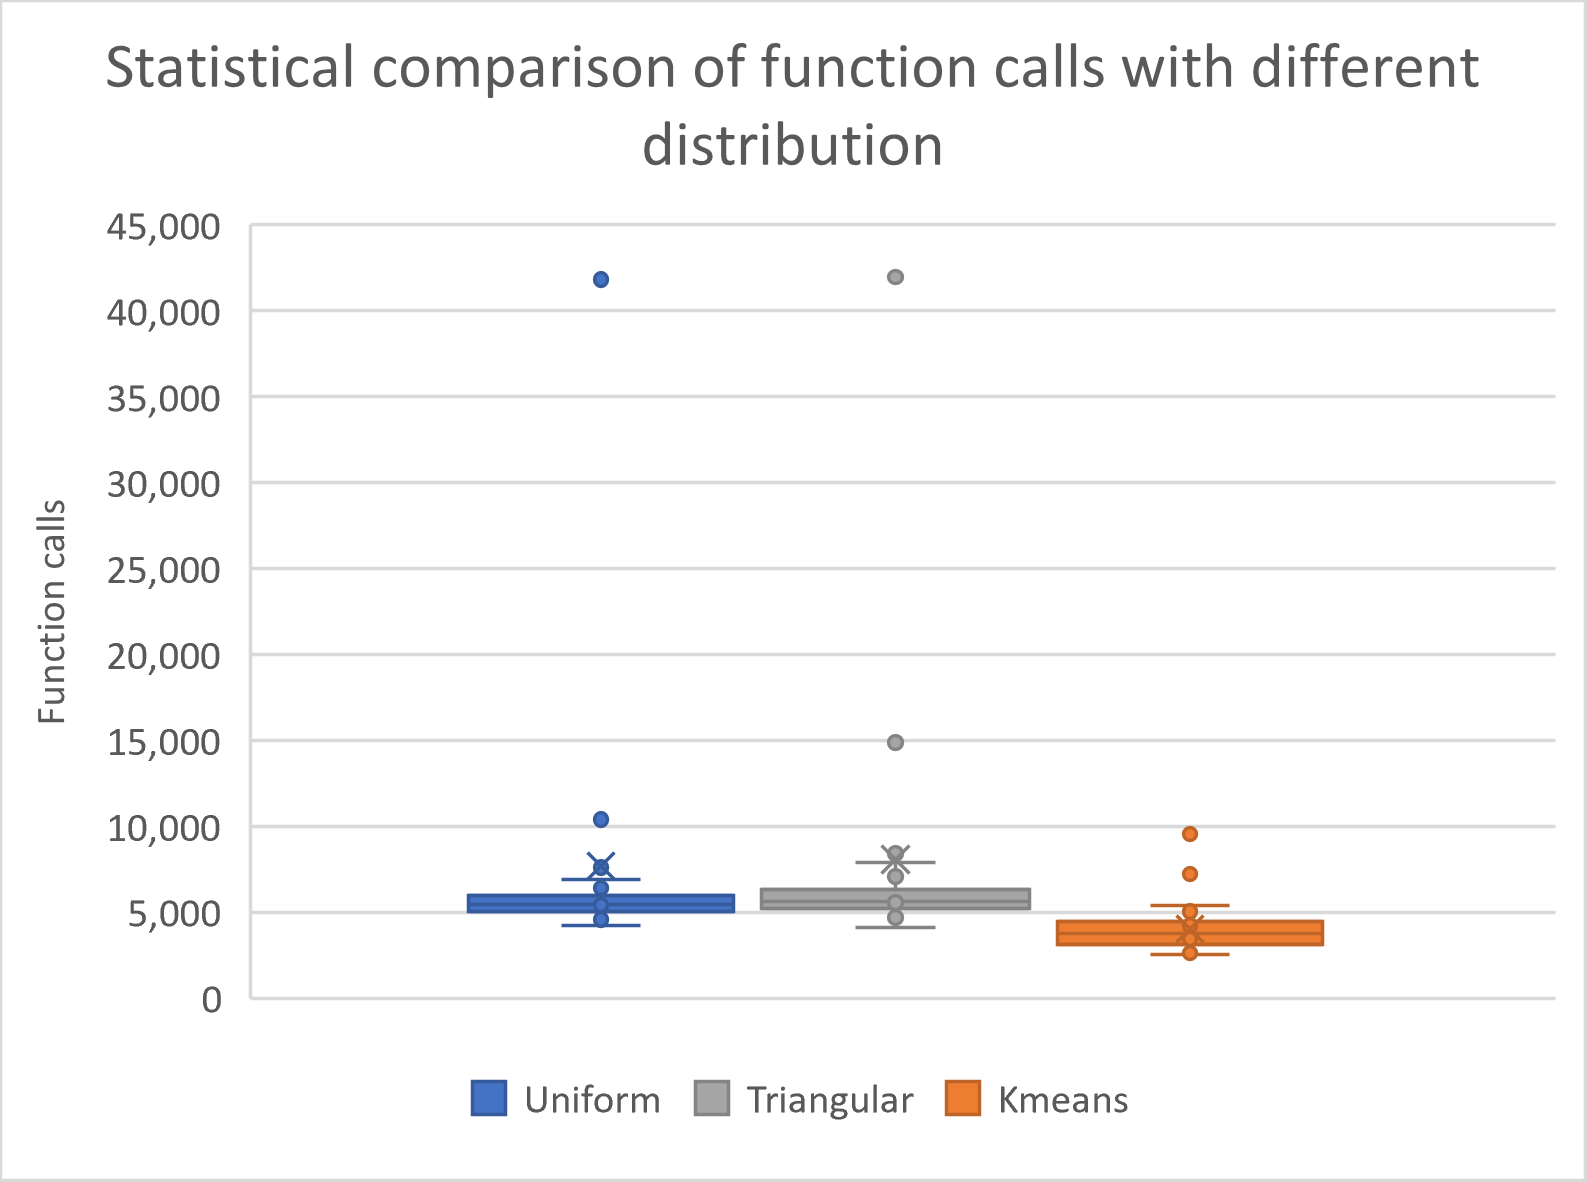
\includegraphics[scale=0.6]{1}\caption{Statistical comparison of function calls with different distribution\label{fig:Statistical-comparison1}}
\end{figure}

\begin{figure}[H]
\begin{centering}
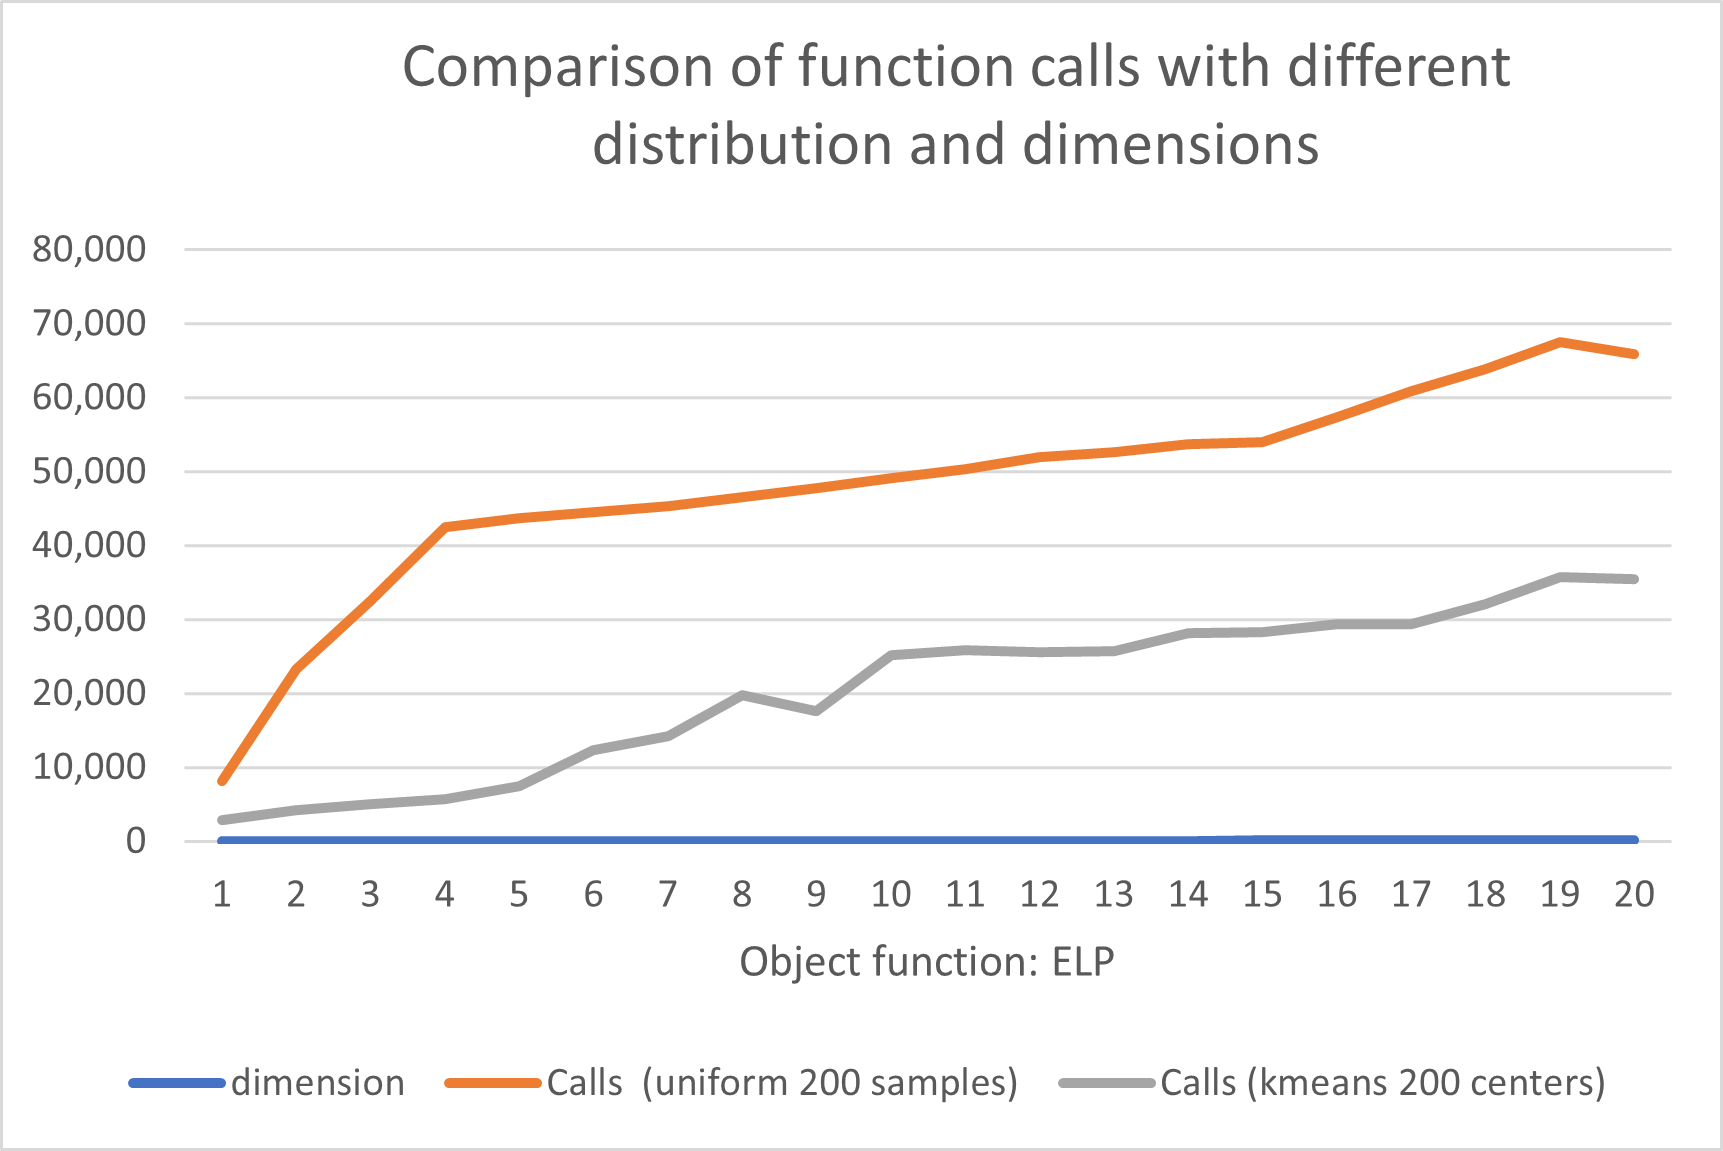
\includegraphics[scale=0.6]{4}
\par\end{centering}
\caption{Comparison of function calls of ELP function with different distributions
and dimensions\label{fig:ComparisonELP}}

\end{figure}

\begin{figure}[H]
\centering{}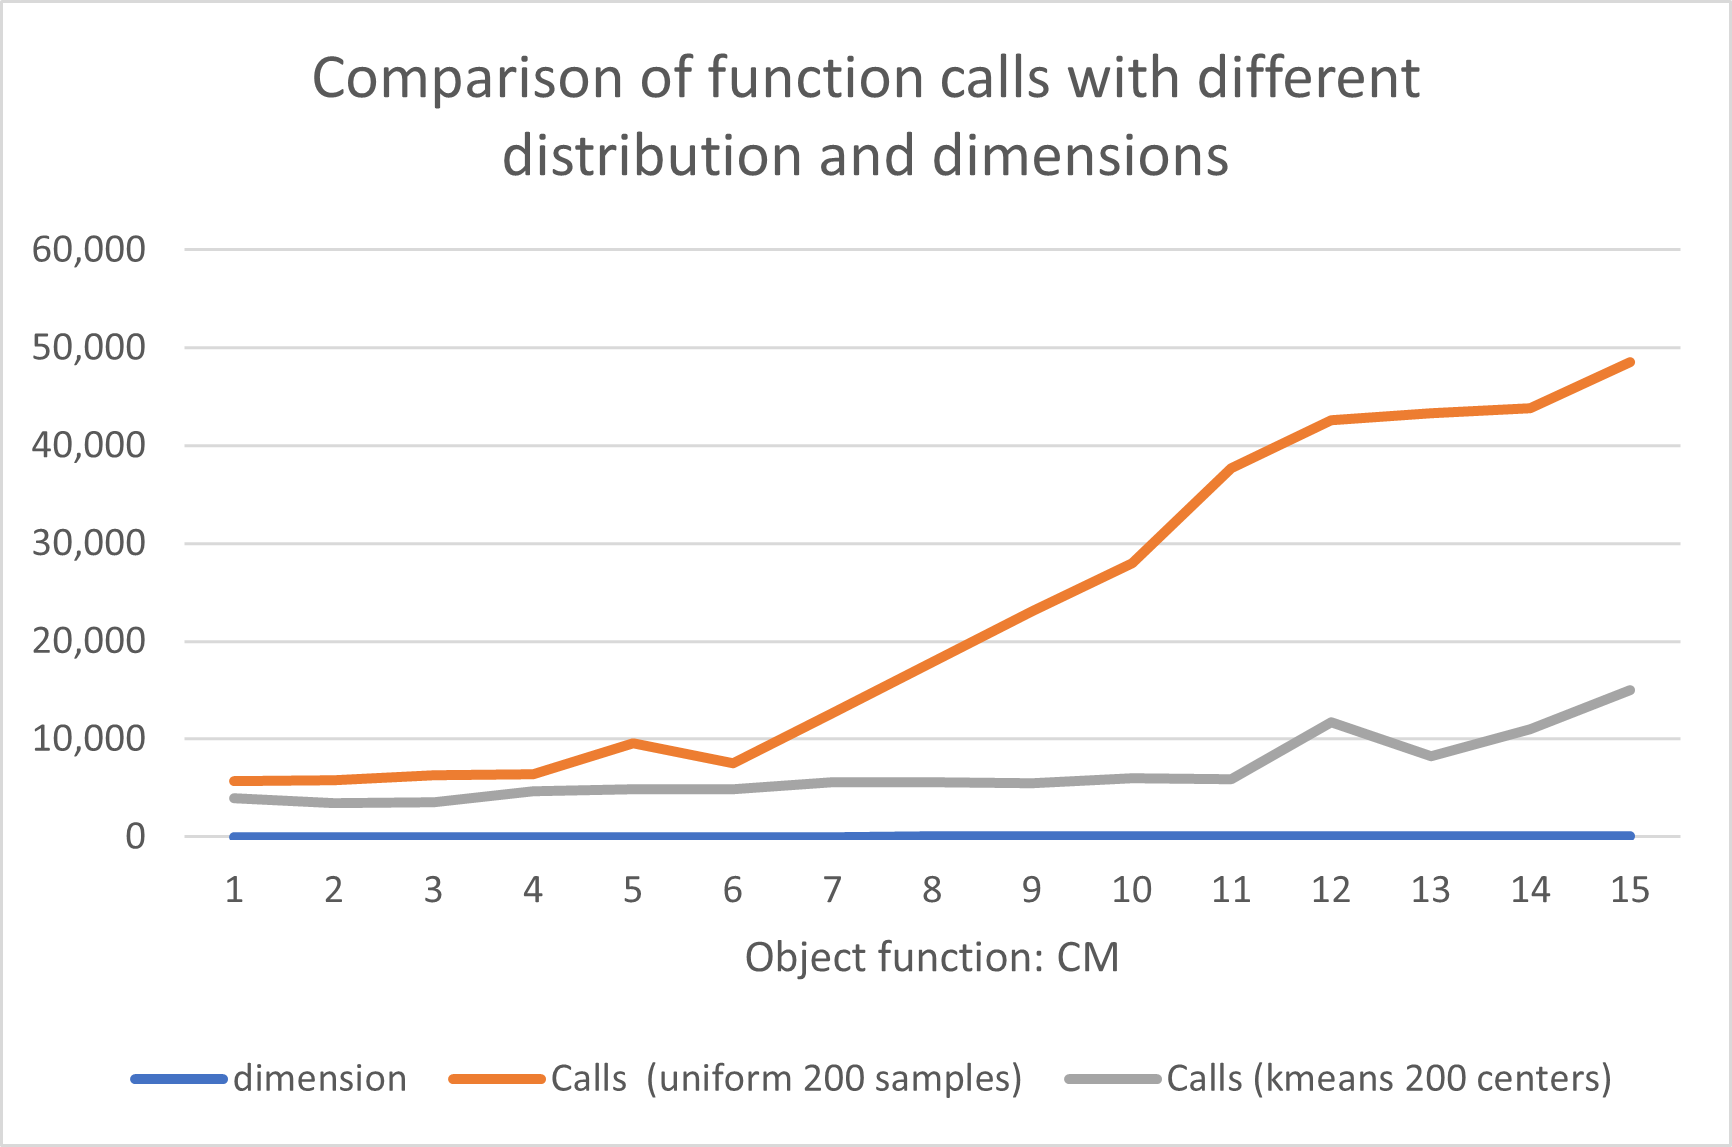
\includegraphics[scale=0.6]{5}\caption{Comparison of function calls of CM function with different distributions
and dimensions\label{fig:ComparisonCM}}
\end{figure}


\section{Conclusions\label{sec:Conclusions}}

In this work, an innovative chromosome initialization method for genetic
algorithms was proposed that utilizes the well-known k-means technique.
These genetic algorithms are used to find the global minimum of multidimensional
functions. This method replaces the initialization of chromosomes
in genetic algorithms which is traditionally performed by some random
distribution with centers produced by the k-means technique. In addition,
in this technique, centers that are close enough are rejected from
being genetic algorithm chromosomes. The above procedure significantly
reduced the required number of function calls compared to random distributions
and furthermore, in difficult high-dimensional functions, it appears
to be a more efficient technique at finding the global minimum than
random distributions. Future research may include incorporation of
parallel techniques such as MPI \citep{openmpi} or OpenMP \citep{openmp}
to speed up the method or application of the initialization process
to other stochastic techniques such as Particle Swarm Optimization
or Differential Evolution.

\vspace{6pt}


\authorcontributions{V.C., I.G.T. and V.S. conceived the idea and methodology and supervised
the technical part regarding the software. V.C. conducted the experiments,
employing several datasets, and provided the comparative experiments.
I.G.T. performed the statistical analysis. V.S. and all other authors
prepared the manuscript. All authors have read and agreed to the published
version of the manuscript.}

\funding{This research received no external funding.}

\institutionalreview{Not applicable.}

\informedconsent{Not applicable. }

\institutionalreview{Not applicable.}

\acknowledgments{The experiments of this research work were performed at the high
performance computing system established at Knowledge and Intelligent
Computing Laboratory, Department of Informatics and Telecommunications,
University of Ioannina, acquired with the project \textquotedblleft Educational
Laboratory equipment of TEI of Epirus\textquotedblright{} with MIS
5007094 funded by the Operational Programme \textquotedblleft Epirus\textquotedblright{}
2014--2020, by ERDF and national funds.}

\conflictsofinterest{The authors declare no conflict of interest.}

\sampleavailability{Not applicable.}

\appendixtitles{no}

\reftitle{References}
\begin{thebibliography}{99}
\bibitem{go_physics1}L. Yang, D. Robin, F. Sannibale, C. Steier,
W. Wan, Global optimization of an accelerator lattice using multiobjective
genetic algorithms, Nuclear Instruments and Methods in Physics Research
Section A: Accelerators, Spectrometers, Detectors and Associated Equipment
\textbf{609}, pp. 50-57, 2009.

\bibitem{go_physics2}E. Iuliano, Global optimization of benchmark
aerodynamic cases using physics-based surrogate models, Aerospace
Science and Technology \textbf{67}, pp.273-286, 2017.

\bibitem{go_physics3}Q. Duan, S. Sorooshian, V. Gupta, Effective
and efficient global optimization for conceptual rainfall-runoff models,
Water Resources Research \textbf{28}, pp. 1015-1031 , 1992.

\bibitem{go_chem1}S. Heiles, R. L. Johnston, Global optimization
of clusters using electronic structure methods, Int. J. Quantum Chem.
\textbf{113}, pp. 2091-- 2109, 2013.

\bibitem{go_chem2}W.H. Shin, J.K. Kim, D.S. Kim, C. Seok, GalaxyDock2:
Protein--ligand docking using beta-complex and global optimization,
J. Comput. Chem. \textbf{34}, pp. 2647-- 2656, 2013.

\bibitem{go_chem3}A. Liwo, J. Lee, D.R. Ripoll, J. Pillardy, H. A.
Scheraga, Protein structure prediction by global optimization of a
potential energy function, Biophysics \textbf{96}, pp. 5482-5485,
1999.

\bibitem{go_econ1}Zwe-Lee Gaing, Particle swarm optimization to solving
the economic dispatch considering the generator constraints, IEEE
Transactions on \textbf{18} Power Systems, pp. 1187-1195, 2003.

\bibitem{go_econ2}C. D. Maranas, I. P. Androulakis, C. A. Floudas,
A. J. Berger, J. M. Mulvey, Solving long-term financial planning problems
via global optimization, Journal of Economic Dynamics and Control
\textbf{21}, pp. 1405-1425, 1997.

\bibitem{go_med1}Eva K. Lee, Large-Scale Optimization-Based Classification
Models in Medicine and Biology, Annals of Biomedical Engineering \textbf{35},
pp 1095-1109, 2007.

\bibitem{go_med2}Y. Cherruault, Global optimization in biology and
medicine, Mathematical and Computer Modelling \textbf{20}, pp. 119-132,
1994.

\bibitem{interval1}M.A. Wolfe, Interval methods for global optimization,
Applied Mathematics and Computation \textbf{75}, pp. 179-206, 1996.

\bibitem{interval2}T. Csendes and D. Ratz, Subdivision Direction
Selection in Interval Methods for Global Optimization, SIAM J. Numer.
Anal. \textbf{34}, pp. 922--938, 1997. 

\bibitem{crs1}W. L. Price, Global optimization by controlled random
search, Journal of Optimization Theory and Applications \textbf{40},
pp. 333-348, 1983.

\bibitem{crs2}Ivan Krivy, Josef Tvrdik, The controlled random search
algorithm in optimizing regression models, Computational Statistics
\& Data Analysis \textbf{20}, pp. 229-234, 1995.

\bibitem{crs3}M.M. Ali, A. Torn, and S. Viitanen, A Numerical Comparison
of Some Modified Controlled Random Search Algorithms, Journal of Global
Optimization \textbf{11},pp. 377--385,1997.

\bibitem{simann_major}S. Kirkpatrick, CD Gelatt, , MP Vecchi, Optimization
by simulated annealing, Science \textbf{220}, pp. 671-680, 1983.

\bibitem{simann1}L. Ingber, Very fast simulated re-annealing, Mathematical
and Computer Modelling \textbf{12}, pp. 967-973, 1989.

\bibitem{simann2}R.W. Eglese, Simulated annealing: A tool for operational
research, Simulated annealing: A tool for operational research \textbf{46},
pp. 271-281, 1990.

\bibitem{diffe1}R. Storn, K. Price, Differential Evolution - A Simple
and Efficient Heuristic for Global Optimization over Continuous Spaces,
Journal of Global Optimization \textbf{11}, pp. 341-359, 1997.

\bibitem{diffe2}J. Liu, J. Lampinen, A Fuzzy Adaptive Differential
Evolution Algorithm. Soft Comput \textbf{9}, pp.448--462, 2005.

\bibitem{pso_major}J. Kennedy and R. Eberhart, \textquotedbl Particle
swarm optimization,\textquotedbl{} Proceedings of ICNN'95 - International
Conference on Neural Networks, 1995, pp. 1942-1948 vol.4, doi: 10.1109/ICNN.1995.488968.

\bibitem{pso1}Riccardo Poli, James Kennedy kennedy, Tim Blackwell,
Particle swarm optimization An Overview, Swarm Intelligence \textbf{1},
pp 33-57, 2007. 

\bibitem{pso2}Ioan Cristian Trelea, The particle swarm optimization
algorithm: convergence analysis and parameter selection, Information
Processing Letters \textbf{85}, pp. 317-325, 2003.

\bibitem{aco1}M. Dorigo, M. Birattari and T. Stutzle, Ant colony
optimization, IEEE Computational Intelligence Magazine \textbf{1},
pp. 28-39, 2006.

\bibitem{aco2}K. Socha, M. Dorigo, Ant colony optimization for continuous
domains, European Journal of Operational Research 185, pp. 1155-1173,
2008.

\bibitem{mshybrid1}M. Perez, F. Almeida and J. M. Moreno-Vega, \textquotedbl Genetic
algorithm with multistart search for the p-Hub median problem,\textquotedbl{}
Proceedings. 24th EUROMICRO Conference (Cat. No.98EX204), Vasteras,
Sweden, 1998, pp. 702-707 vol.2.

\bibitem{mshybrid2}H. C. B. d. Oliveira, G. C. Vasconcelos and G.
B. Alvarenga, \textquotedbl A Multi-Start Simulated Annealing Algorithm
for the Vehicle Routing Problem with Time Windows,\textquotedbl{}
2006 Ninth Brazilian Symposium on Neural Networks (SBRN'06), Ribeirao
Preto, Brazil, 2006, pp. 137-142.

\bibitem{psohybrid1}B. Liu, L. Wang, Y.H. Jin, F. Tang, D.X. Huang,
Improved particle swarm optimization combined with chaos, Chaos Solitons
and Fractals \textbf{25}, pp. 1261-1271, 2005.

\bibitem{psohybrid2}X.H. Shi, Y.C. Liang, H.P. Lee, C. Lu, L.M. Wang,
An improved GA and a novel PSO-GA based hybrid algorithm, Information
Processing Letters \textbf{93}, pp. 255-261, 2005.

\bibitem{psohybrid3}Harish Garg, A hybrid PSO-GA algorithm for constrained
optimization problems, Applied Mathematics and Computation \textbf{274},
pp. 292-305, 2016.

\bibitem{parallel-multistart}J. Larson and S.M. Wild, Asynchronously
parallel optimization solver for finding multiple minima, Mathematical
Programming Computation \textbf{10}, pp. 303-332, 2018.

\bibitem{parallel-multistart2}H.P.J. Bolton, J.F. Schutte, A.A. Groenwold,
Multiple Parallel Local Searches in Global Optimization. In: Dongarra
J., Kacsuk P., Podhorszki N. (eds) Recent Advances in Parallel Virtual
Machine and Message Passing Interface. EuroPVM/MPI 2000. Lecture Notes
in Computer Science, vol 1908. Springer, Berlin, Heidelberg, 2000.

\bibitem{msgpu1}R. Kamil, S. Reiji, An Efficient GPU Implementation
of a Multi-Start TSP Solver for Large Problem Instances, Proceedings
of the 14th Annual Conference Companion on Genetic and Evolutionary
Computation, pp. 1441-1442, 2012.

\bibitem{msgpu2}Van Luong T., Melab N., Talbi EG. (2011) GPU-Based
Multi-start Local Search Algorithms. In: Coello C.A.C. (eds) Learning
and Intelligent Optimization. LION 2011. Lecture Notes in Computer
Science, vol 6683. Springer, Berlin, Heidelberg. https://doi.org/10.1007/978-3-642-25566-3\_24

\bibitem{Holland1}J.H. Holland, Genetic algorithms. Scientific american
\textbf{267}, pp. 66-73, 1992.

\bibitem{Stender}J. Stender, Parallel Genetic Algorithms:Theory \&
Applications. Edition: IOS Press, 1993. 

\bibitem{genetic1}D. Goldberg, Genetic Algorithms in Search, Optimization
and Machine Learning, Addison-Wesley Publishing Company, Reading,
Massachussets, 1989.

\bibitem{genetic2}Z. Michaelewicz, Genetic Algorithms + Data Structures
= Evolution Programs. Springer - Verlag, Berlin, 1996.

\bibitem{Ansari}S. Ansari, K. Alnajjar, M. Saad, S. Abdallah, A.
Moursy, Automatic Digital Modulation Recognition Based on Genetic-Algorithm-Optimized
Machine Learning Models, IEEE Access \textbf{10}, pp. 50265-50277,
2022.

\bibitem{Ji}Y. Ji, S. Liu, M. Zhou, Z. Zhao, X. Guo, L. Qi, L., A
machine learning and genetic algorithm-based method for predicting
width deviation of hot-rolled strip in steel production systems. Information
Sciences \textbf{589}, pp. 360-375, 2022.

\bibitem{Santana}Y. Hervis Santana, R. Martinez Alonso, G. Guillen
Nieto, L. Martens, W. Joseph, D. Plets, Indoor genetic algorithm-based
5G network planning using a machine learning model for path loss estimation.
Applied Sciences \textbf{12}, 3923, 2022.

\bibitem{Liu}X. Liu, D. Jiang, B. Tao, G. Jiang, Y. Sun, J. Kong,
B. Chen, Genetic algorithm-based trajectory optimization for digital
twin robots. Frontiers in Bioengineering and Biotechnology \textbf{9},
793782, 2022.

\bibitem{Nonoyama}K. Nonoyama, Z. Liu, T. Fujiwara, M.M. Alam, T.
Nishi, Energy-efficient robot configuration and motion planning using
genetic algorithm and particle swarm optimization. Energies \textbf{15},
2074, 2022.

\bibitem{LiuK}K. Liu, B. Deng, Q. Shen, J. Yang, Y. Li, Optimization
based on genetic algorithms on energy conservation potential of a
high speed SI engine fueled with butanol--gasoline blends, Energy
Reports \textbf{8}, pp. 69-80, 2022.

\bibitem{Zhou}G. Zhou, Z. Zhu, S. Luo, Location optimization of electric
vehicle charging stations: Based on cost model and genetic algorithm,
Energy \textbf{247}, 123437, 2022.

\bibitem{Chen}Q. Chen, X. Hu, Design of intelligent control system
for agricultural greenhouses based on adaptive improved genetic algorithm
for multi-energy supply system, Energy Reports \textbf{8}, pp. 12126-12138,
2022.

\bibitem{Min}D. Min, Z. Song, H. Chen, T. Wang, T. Zhang, Genetic
algorithm optimized neural network based fuel cell hybrid electric
vehicle energy management strategy under start-stop condition, Applied
Energy \textbf{306}, 118036, 2022.

\bibitem{Doewes}R.I. Doewes, R. Nair, T. Sharma, Diagnosis of COVID-19
through blood sample using ensemble genetic algorithms and machine
learning classifier, World Journal of Engineering \textbf{19}, pp.
175-182, 2022.

\bibitem{Choudhury}S. Choudhury, M. Rana, A. Chakraborty, S. Majumder,
S. Roy, A. RoyChowdhury, S. Datta, Design of patient specific basal
dental implant using Finite Element method and Artificial Neural Network
technique. Journal of Engineering in Medicine \textbf{236}, pp. 1375-1387,
2022. 

\bibitem{ElAnwar}M.I. El-Anwar, M.M. El-Zawahry, A three dimensional
finite element study on dental implant design, Journal of Genetic
Engineering and Biotechnology \textbf{9}, pp. 77-82, 2011.

\bibitem{Zheng}Zheng, Q. \& Zhong, J. (2022). Design of Automatic
Pronunciation Error Correction System for Cochlear Implant Based on
Genetic Algorithm. ICMMIA: Application of Intelligent Systems in Multi-modal
Information Analytics pp 1041--1047. 

\bibitem{Brahim}O. Brahim, B. Hamid, N. Mohammed, Optimal design
of inductive coupled coils for biomedical implants using metaheuristic
techniques. E3S Web Conf.: Volume 351, 2022.

\bibitem{Tokgoz}E. Tokgoz, M.A. Carro, Applications of Artificial
Intelligence, Machine Learning, and Deep Learning on Facial Plastic
Surgeries. Springer: Cosmetic and Reconstructive Facial Plastic Surgery
pp 281--306, 2023.

\bibitem{Wang}B. Wang, J.F. Gomez-Aguilar, Z. Sabir, M.A.Z. Raja,
W. Xia, H. Jahanshahi, M.O. Alassafi, F. Alsaadi, Surgery Using The
Capability Of Morlet Wavelet Artificial Neural Networks, Fractals\textbf{
30}, 2240147, 2023.

\bibitem{kmeansNew}M. Ahmed, R. Seraj, S.M.S. Islam, The k-means
algorithm: A comprehensive survey and performance evaluation, Electronics
\textbf{9}, 1295, 2020.

\bibitem{gainit1}H. Maaranen, K. Miettinen, M.M. Makela, Quasi-random
initial population for genetic algorithms. Computers \& Mathematics
with Applications \textbf{47}, pp. 1885-1895, 2004.

\bibitem{gainit2}P.V. Paul, P. Dhavachelvan, R. Baskaran, A novel
population initialization technique for Genetic Algorithm, In: 2013
International Conference on Circuits, Power and Computing Technologies
(ICCPCT), Nagercoil, India, pp. 1235-1238, 2013.

\bibitem{gainit3}C. Li, X. Chu, Y. Chen, L. Xing, A knowledge-based
technique for initializing a genetic algorithm. Journal of Intelligent
\& Fuzzy Systems \textbf{31}, pp. 1145-1152, 2016.

\bibitem{gainit4}A.B. Hassanat, V.S. Prasath, M.A. Abbadi, S.A. Abu-Qdari,
H. Faris, An improved genetic algorithm with a new initialization
mechanism based on regression techniques. Information \textbf{9},
167, 2018.

\bibitem{kaelo}P. Kaelo, M.M. Ali, Integrated crossover rules in
real coded genetic algorithms, European Journal of Operational Research
\textbf{176}, pp. 60-76, 2007.

\bibitem{Tsoulos1}I.G. Tsoulos, Modifications of real code genetic
algorithm for global optimization, Applied Mathematics and Computation
\textbf{203}, pp. 598-607, 2008.

\bibitem{Powell}M.J.D Powell, A Tolerant Algorithm for Linearly Constrained
Optimization Calculations, Mathematical Programming \textbf{45}, pp.
547-566, 1989. 

\bibitem{Kennedy}J. Kennedy, R. Eberhart, Particle swarm optimization,
In: Proceedings of IEEE International Conference on Neural Networks
pp. 1942-1948, 1995.

\bibitem{Beyer}H.G. Beyer, H.P. Schwefel, Evolution strategies--A
comprehensive introduction, Natural Computing \textbf{1}, pp. 3-52,
2002.

\bibitem{LeCun}Y. LeCun, Y. Bengio, G. Hinton, Deep learning, Nature
\textbf{521}, pp. 436-444, 2015.

\bibitem{Holland3}J.H. Holland, Adaptation in Natural and Artificial
Systems, University of Michigan Press, 1975.

\bibitem{Whitley}D. Whitley, The GENITOR algorithm and selection
pressure: Why rank-based allocation of reproductive trials is best,
In Proceedings of the Third International Conference on Genetic Algorithms,
pp. 116-121, 1994.

\bibitem{Eiben}A.E. Eiben, J.E. Smith, Introduction to Evolutionary
Computing, Springer, 2015.

\bibitem{Lloyd}S. Lloyd, Least squares quantization in PCM, IEEE
Transactions on Information Theory \textbf{28}, pp. 129--137, 1982.

\bibitem{MacQueen}J.B. MacQueen, Some Methods for classification
and Analysis of Multivariate Observations. Proceedings of 5th Berkeley
Symposium on Mathematical Statistics and Probability. Vol. 1. University
of California Press. pp. 281--297. MR 0214227. Zbl 0214.46201, 1967.

\bibitem{Jain}A.K. Jain, M.N. Murty, P.J. Flynn, Data clustering:
A review, ACM Computing Surveys \textbf{31}, pp. 264-323, 1999.

\bibitem{Bishop}C.M. Bishop, Pattern recognition and machine learning,
Springer, 2006. 

\bibitem{Hastie}T. Hastie, R. Tibshirani, J. Friedman, The elements
of statistical learning: Data mining, inference, and prediction, Springer,
2009.

\bibitem{Ali1}M. Montaz Ali, Charoenchai Khompatraporn, Zelda B.
Zabinsky, A Numerical Evaluation of Several Stochastic Algorithms
on Selected Continuous Global Optimization Test Problems, Journal
of Global Optimization \textbf{31}, pp 635-672, 2005. 

\bibitem{Floudas1}C.A. Floudas, P.M. Pardalos, C. Adjiman, W. Esposoto,
Z. G$\ddot{\mbox{u}}$m$\ddot{\mbox{u}}$s, S. Harding, J. Klepeis,
C. Meyer, C. Schweiger, Handbook of Test Problems in Local and Global
Optimization, Kluwer Academic Publishers, Dordrecht, 1999.

\bibitem{gkls}M. Gaviano, D.E. Ksasov, D. Lera, Y.D. Sergeyev, Software
for generation of classes of test functions with known local and global
minima for global optimization, ACM Trans. Math. Softw. \textbf{29},
pp. 469-480, 2003.

\bibitem{Jones}J.E. Lennard-Jones, On the Determination of Molecular
Fields, Proc. R. Soc. Lond. A \textbf{ 106}, pp. 463--477, 1924.

\bibitem{triangular}W.E. Stein, M.F. Keblis, A new method to simulate
the triangular distribution, Mathematical and Computer Modelling Volume
\textbf{49}, pp. 1143-1147, 2009.

\bibitem{openmpi}W. Gropp, E. Lusk, N. Doss, A. Skjellum, A high-performance,
portable implementation of the MPI message passing interface standard,
Parallel Computing \textbf{22}, pp. 789-828, 1996.

\bibitem{openmp}R. Chandra, L. Dagum, D. Kohr, D. Maydan,J. McDonald
and R. Menon, Parallel Programming in OpenMP, Morgan Kaufmann Publishers
Inc., 2001.

\end{thebibliography}

\end{document}
